% ══════════════════════════════════════════════════════════════════════
% StenoWav — User Guide
% ══════════════════════════════════════════════════════════════════════
\documentclass[11pt,a4paper]{article}

\usepackage[utf8]{inputenc}
\usepackage[T1]{fontenc}
\usepackage{amsmath}
\usepackage{hyperref}
\usepackage{geometry}
\usepackage{booktabs}
\usepackage{enumitem}
\usepackage{tikz}
\usepackage{xcolor}
\usepackage{listings}
\usepackage{fancyhdr}
\usepackage{tcolorbox}
\usepackage{graphicx}

\geometry{margin=2.5cm, headheight=14.5pt}
\hypersetup{colorlinks=true, linkcolor=blue!60!black, urlcolor=blue!60!black}

\pagestyle{fancy}
\fancyhf{}
\rhead{\textit{StenoWav User Guide}}
\lhead{\textit{\nouppercase{\leftmark}}}
\rfoot{\thepage}

\definecolor{rustbg}{RGB}{245,245,240}
\definecolor{rustkw}{RGB}{180,60,30}
\definecolor{ruststr}{RGB}{40,120,40}
\definecolor{rustcmt}{RGB}{120,120,120}

\lstdefinestyle{rust}{
    language={},
    basicstyle=\ttfamily\small,
    breaklines=true,
    frame=single,
    framesep=4pt,
    backgroundcolor=\color{rustbg},
    keywordstyle=\color{rustkw}\bfseries,
    stringstyle=\color{ruststr},
    commentstyle=\color{rustcmt}\itshape,
    morekeywords={let,mut,fn,use,pub,struct,impl,const,mod,match,if,else,for,in,return,Ok,Err},
    morestring=[b]",
    morecomment=[l]{//},
}

\newtcolorbox{infobox}[1][]{
    colback=blue!5!white,
    colframe=blue!50!black,
    fonttitle=\bfseries,
    title=#1,
    arc=2mm,
}

\newtcolorbox{warnbox}[1][]{
    colback=orange!5!white,
    colframe=orange!60!black,
    fonttitle=\bfseries,
    title=#1,
    arc=2mm,
}

\title{
    \textbf{StenoWav} \\[0.5em]
    \Large User Guide \\[0.3em]
    \normalsize Version 0.1.0
}
\author{StenoWav Project}
\date{March 2026}

\begin{document}
\maketitle
\tableofcontents
\newpage

% ──────────────────────────────────────────────────────────────────
\section{What Is StenoWav?}
% ──────────────────────────────────────────────────────────────────

StenoWav hides secret data inside ordinary audio files.  You give it a
WAV file, a message (any bytes), and a secret key.  It gives you back a
WAV file that sounds exactly the same --- but carries your message inside
it.  Anyone with the same key can extract the message; everyone else
just hears music.

This is called \textbf{audio steganography}: hiding information inside
audio in a way that is invisible to the ear and difficult to detect
without the key.

\subsection{Key Features}

\begin{itemize}
    \item \textbf{Two embedding modes}: hide data directly in audio
          samples (time domain) or in the frequency spectrum.
    \item \textbf{Smart placement}: the framework analyses the audio
          and only hides data in loud sections, where small changes
          are masked by the music itself.
    \item \textbf{Encryption}: each packet of hidden data is encrypted
          with a unique cipher derived from the audio itself.
    \item \textbf{Self-contained}: the watermarked file contains
          everything needed for extraction --- just provide the key.
    \item \textbf{Optional noise masking}: an extra ``dither'' pass
          makes statistical detection even harder.
    \item \textbf{No Python}: built entirely in Rust and C for
          performance and safety.
\end{itemize}


% ──────────────────────────────────────────────────────────────────
\section{Quick Start}
% ──────────────────────────────────────────────────────────────────

\subsection{Hide a Message}

\begin{lstlisting}[style=rust]
use stenowav::steno::{Steno, StenoConfig};

// Your secret key (32 bytes --- like a password)
let key = [42u8; 32];

// Default settings work out of the box
let config = StenoConfig::default();

// Hide "Hello, world!" inside a WAV file
Steno::encode(
    "original.wav",      // input audio
    "watermarked.wav",   // output audio (sounds the same!)
    b"Hello, world!",    // your secret message
    &key,
    &config,
).unwrap();
\end{lstlisting}

\subsection{Recover the Message}

\begin{lstlisting}[style=rust]
// Same key and config as encoding
let recovered = Steno::decode(
    "watermarked.wav",
    &key,
    &config,
).unwrap();

assert_eq!(recovered, b"Hello, world!");
\end{lstlisting}

That's it.  Two function calls --- one to hide, one to recover.


% ──────────────────────────────────────────────────────────────────
\section{How It Works (The Simple Version)}
% ──────────────────────────────────────────────────────────────────

\subsection{The Basic Idea}

Audio is stored as thousands of numbers per second (called \textbf{samples}).
Each sample represents how loud the sound is at that instant.  For 16-bit
audio, each sample is an integer from $-32768$ to $+32767$.

StenoWav makes tiny changes to some of these numbers.  The changes are so
small that your ears can't tell the difference, but a computer with the
right key can read them back.

\subsection{Step by Step}

\begin{enumerate}
    \item \textbf{Read the audio}: Load the WAV file into memory.

    \item \textbf{Find good hiding spots}: Analyse the audio to find
          the loud sections.  Loud music masks small changes better than
          silence does.  Quiet sections are left untouched.

    \item \textbf{Pick random positions}: Using the secret key as a seed,
          a random number generator picks exactly which samples to modify.
          Without the key, an attacker doesn't know which samples to look at.

    \item \textbf{Create a cipher}: For each chunk of data, 8 ``mask''
          samples are modified to encode a 16-bit encryption key.  This
          key is then used to encrypt the actual data before embedding it.

    \item \textbf{Embed the data}: The encrypted data bits are hidden in
          16 more samples using a technique called QIM, which rounds each
          sample to the nearest value on a mathematical grid that encodes
          the desired bit.

    \item \textbf{Add noise (optional)}: A tiny amount of random noise is
          added to all the \emph{other} samples, so the modified ones
          don't stand out statistically.

    \item \textbf{Write the output}: Save the modified audio as a new WAV
          file.  It sounds identical to the original.
\end{enumerate}

\subsection{Why Is It Secure?}

Three things protect your data:
\begin{itemize}
    \item \textbf{Position}: Without the key, you don't know \emph{which}
          samples carry data.  There could be millions of samples.
    \item \textbf{Encryption}: Even if you found the right samples, the
          data is XOR-encrypted with a cipher derived from the audio itself.
    \item \textbf{Stealth}: With dither enabled, the entire audio has
          micro-noise, so modified and unmodified samples look the same
          under statistical analysis.
\end{itemize}


% ──────────────────────────────────────────────────────────────────
\section{Configuration}
% ──────────────────────────────────────────────────────────────────

StenoWav works out of the box with defaults, but you can tune every
parameter.

\subsection{Choosing a Domain}

\begin{lstlisting}[style=rust]
// Time domain (default) --- modifies audio samples directly
let config = StenoConfig::time();

// Frequency domain --- modifies the frequency spectrum
let config = StenoConfig::frequency();
\end{lstlisting}

\begin{infobox}[Which domain should I use?]
\textbf{Time domain} is simpler and faster.  Good for most use cases.

\textbf{Frequency domain} spreads changes across many time-domain samples
(via the inverse FFT), which can be harder to detect but uses more
computational resources.

Both modes are well-tested and produce inaudible results on typical music.
\end{infobox}

\subsection{Builder Methods}

Chain methods to customise:

\begin{lstlisting}[style=rust]
let config = StenoConfig::time()
    .with_dither()           // enable noise masking
    .with_time_delta(0.01)   // larger step = more robust
    .with_channel(1);        // embed in right channel
\end{lstlisting}

\subsection{All Parameters}

\begin{center}
\begin{tabular}{@{}lcp{7.5cm}@{}}
\toprule
Parameter & Default & What it does \\
\midrule
\texttt{domain} & Time & Where to hide the data \\
\texttt{time\_delta} & 0.005 & Size of the rounding grid (time domain).
    Larger = more robust to noise but slightly more audible \\
\texttt{freq\_delta} & 0.05 & Same but for frequency domain \\
\texttt{rms\_high} & 0.10 & Loudness threshold for ``high power''.
    Sections above this get embedded in \\
\texttt{rms\_low} & 0.01 & Sections below this are skipped entirely \\
\texttt{rms\_segment\_size} & 4096 & How many samples per loudness measurement \\
\texttt{freq\_window\_size} & 1024 & FFT window size (must be a power of 2) \\
\texttt{freq\_min\_bin} & 10 & Skip very low frequencies \\
\texttt{freq\_max\_bin} & 400 & Skip very high frequencies \\
\texttt{dither\_enabled} & false & Add noise to non-data samples \\
\texttt{dither\_intensity} & $\sim$6.1e-5 & How much noise ($\sim$2 least significant bits) \\
\texttt{channel} & 0 & Audio channel (0 = left, 1 = right) \\
\bottomrule
\end{tabular}
\end{center}

\subsection{Direct Field Access}

All fields are public, so you can set them directly too:

\begin{lstlisting}[style=rust]
let mut config = StenoConfig::default();
config.rms_high = 0.15;
config.rms_low = 0.02;
config.dither_enabled = true;
\end{lstlisting}


% ──────────────────────────────────────────────────────────────────
\section{API Reference}
% ──────────────────────────────────────────────────────────────────

\subsection{File-Based API}

These are the main functions most users need:

\begin{tcolorbox}[colback=gray!5, colframe=gray!60, title=\texttt{Steno::encode}]
\begin{lstlisting}[style=rust]
Steno::encode(
    input_path,    // path to source WAV (16-bit PCM)
    output_path,   // path to write watermarked WAV
    data,          // &[u8] --- any bytes you want to hide
    key,           // &[u8; 32] --- your secret key
    config,        // &StenoConfig
) -> Result<(), StenoError>
\end{lstlisting}
\end{tcolorbox}

\begin{tcolorbox}[colback=gray!5, colframe=gray!60, title=\texttt{Steno::decode}]
\begin{lstlisting}[style=rust]
Steno::decode(
    watermarked_path,  // path to watermarked WAV
    key,               // &[u8; 32] --- same key as encoding
    config,            // &StenoConfig --- same config as encoding
) -> Result<Vec<u8>, StenoError>
\end{lstlisting}
\end{tcolorbox}

\subsection{In-Memory API}

For when you already have audio samples loaded:

\begin{tcolorbox}[colback=gray!5, colframe=gray!60, title=\texttt{Steno::encode\_samples} / \texttt{decode\_samples}]
\begin{lstlisting}[style=rust]
// Modify samples in-place
Steno::encode_samples(
    samples,  // &mut [f64] --- audio in [-1.0, 1.0]
    data, key, config,
) -> Result<(), StenoError>

// Extract from samples
Steno::decode_samples(
    samples,  // &[f64]
    key, config,
) -> Result<Vec<u8>, StenoError>
\end{lstlisting}
\end{tcolorbox}

\subsection{Error Handling}

All functions return \texttt{Result} with \texttt{StenoError}:

\begin{itemize}
    \item \texttt{StenoError::Wav} --- file not found, not a valid WAV, etc.
    \item \texttt{StenoError::Embed} --- audio too short/quiet, wrong key, etc.
    \item \texttt{StenoError::Config} --- invalid parameters
          (negative delta, non-power-of-2 window, etc.)
\end{itemize}

\begin{warnbox}[Wrong key behaviour]
If you try to decode with the wrong key, you get an error (not garbage data).
The framework checks for a magic signature in the header --- a wrong key
produces an invalid signature and returns
\texttt{StenoError::Embed(InvalidConfig(...))}.
\end{warnbox}


% ──────────────────────────────────────────────────────────────────
\section{Architecture Overview}
% ──────────────────────────────────────────────────────────────────

StenoWav is built in layers, each handling one concern:

\begin{center}
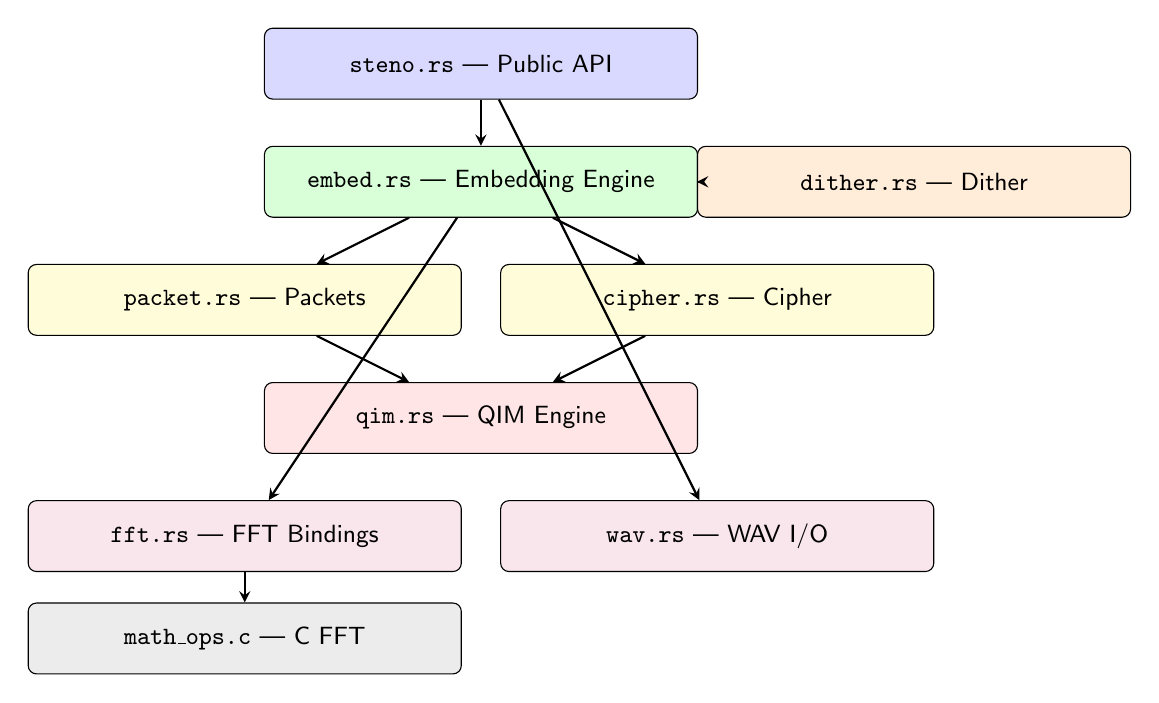
\begin{tikzpicture}[
    box/.style={draw, rounded corners=3pt, minimum width=5.5cm,
                minimum height=0.9cm, fill=#1, font=\small\sffamily},
    arr/.style={->, thick, >=stealth},
]
    \node[box=blue!15]    (steno)  at (0, 6.0) {\texttt{steno.rs} --- Public API};
    \node[box=green!15]   (embed)  at (0, 4.5) {\texttt{embed.rs} --- Embedding Engine};
    \node[box=yellow!15]  (packet) at (-3, 3.0) {\texttt{packet.rs} --- Packets};
    \node[box=yellow!15]  (cipher) at ( 3, 3.0) {\texttt{cipher.rs} --- Cipher};
    \node[box=orange!15]  (dither) at ( 5.5, 4.5) {\texttt{dither.rs} --- Dither};
    \node[box=red!10]     (qim)    at (0, 1.5) {\texttt{qim.rs} --- QIM Engine};
    \node[box=purple!10]  (fft)    at (-3, 0) {\texttt{fft.rs} --- FFT Bindings};
    \node[box=purple!10]  (wav)    at ( 3, 0) {\texttt{wav.rs} --- WAV I/O};
    \node[box=gray!15]    (c)      at (-3, -1.3) {\texttt{math\_ops.c} --- C FFT};

    \draw[arr] (steno)  -- (embed);
    \draw[arr] (steno)  -- (wav);
    \draw[arr] (embed)  -- (packet);
    \draw[arr] (embed)  -- (cipher);
    \draw[arr] (embed)  -- (dither);
    \draw[arr] (embed)  -- (fft);
    \draw[arr] (packet) -- (qim);
    \draw[arr] (cipher) -- (qim);
    \draw[arr] (fft)    -- (c);
\end{tikzpicture}
\end{center}

\begin{description}[style=nextline]
    \item[\texttt{steno.rs}] The front door.  Handles file I/O, config
        validation, channel selection.  Everything goes through here.
    \item[\texttt{embed.rs}] The brain.  Decides where to embed (RMS
        analysis), manages headers, dispatches to time or frequency path.
    \item[\texttt{packet.rs}] The workhorse.  Selects random sample
        positions, encodes/decodes individual packets.
    \item[\texttt{cipher.rs}] The locksmith.  Generates and extracts
        per-packet encryption keys from mask samples.
    \item[\texttt{qim.rs}] The math.  The core quantisation algorithm
        that turns a sample and a bit into a modified sample.
    \item[\texttt{dither.rs}] The camouflage.  Adds inaudible noise to
        non-payload samples.  Also provides quality metrics (SNR, etc.).
    \item[\texttt{fft.rs}] The bridge.  Safe Rust wrappers around the
        C FFT library.
    \item[\texttt{wav.rs}] The translator.  Reads and writes 16-bit PCM
        WAV files to/from \texttt{f64} sample arrays.
    \item[\texttt{math\_ops.c}] The engine room.  Radix-2 Cooley-Tukey
        FFT in pure C.
\end{description}


% ──────────────────────────────────────────────────────────────────
\section{Understanding QIM (Simplified)}
% ──────────────────────────────────────────────────────────────────

Imagine a number line with marks every 0.01 units:
\[
    \ldots, -0.02, -0.01, \; 0.00, \; 0.01, \; 0.02, \; 0.03, \ldots
\]

Now colour the marks alternately: \textbf{blue} (even index) and
\textbf{red} (odd index):
\[
    \ldots,
    \textcolor{blue}{-0.02},
    \textcolor{red}{-0.01},
    \textcolor{blue}{0.00},
    \textcolor{red}{0.01},
    \textcolor{blue}{0.02},
    \textcolor{red}{0.03},
    \ldots
\]

To hide a \textbf{0}, round the sample to the nearest \textcolor{blue}{blue} mark.
To hide a \textbf{1}, round it to the nearest \textcolor{red}{red} mark.

To read the bit back, round the sample and check its colour.

That's QIM.  The spacing (0.01 in this example) is called \textbf{delta}
($\Delta$).  Bigger delta = the mark is harder to accidentally knock off
(more robust), but the rounding changes are bigger (more audible).


% ──────────────────────────────────────────────────────────────────
\section{Practical Guidelines}
% ──────────────────────────────────────────────────────────────────

\subsection{Audio Requirements}

\begin{itemize}
    \item \textbf{Format}: 16-bit PCM WAV (mono or stereo, any sample rate).
    \item \textbf{Length}: Longer audio = more room for data.
          At least a few seconds of music for short messages.
    \item \textbf{Content}: Music with dynamic range works best.
          Pure silence or very quiet recordings have fewer eligible
          hiding spots.
\end{itemize}

\subsection{How Much Data Can I Hide?}

Each ``packet'' carries 2 bytes and uses about 24 sample positions.
The framework also needs 7 packets for its internal header.

\begin{center}
\begin{tabular}{@{}rr@{}}
\toprule
Audio length (44.1 kHz mono) & Approximate capacity \\
\midrule
10 seconds ($\sim$441K samples) & $\sim$700 bytes \\
1 minute ($\sim$2.6M samples) & $\sim$4 KB \\
3 minutes ($\sim$7.9M samples) & $\sim$14 KB \\
\bottomrule
\end{tabular}
\end{center}

\begin{warnbox}[Capacity depends on content]
These numbers assume roughly half the audio is ``loud enough'' for
embedding.  Quiet recordings or recordings with lots of silence
will have lower capacity.
\end{warnbox}

\subsection{Choosing Delta}

\begin{center}
\begin{tabular}{@{}lll@{}}
\toprule
Delta & Robustness & Audibility \\
\midrule
0.003 & Lower (fragile) & Very imperceptible \\
0.005 & Good (default) & Imperceptible \\
0.01  & High & Still imperceptible \\
0.02  & Very high & Borderline (quiet passages) \\
\bottomrule
\end{tabular}
\end{center}

The default (0.005) is a safe all-rounder.  Only increase it if you
need extra robustness against noise or processing.

\subsection{Key Management}

\begin{itemize}
    \item The key is 32 bytes (256 bits).  Use a cryptographically
          secure random generator to create it.
    \item Both encoder and decoder must use \textbf{exactly the same
          key and config}.  Any mismatch will fail.
    \item Store keys securely --- anyone with the key can extract
          the hidden data.
\end{itemize}


% ──────────────────────────────────────────────────────────────────
\section{Examples}
% ──────────────────────────────────────────────────────────────────

\subsection{Hide a Text Message}

\begin{lstlisting}[style=rust]
use stenowav::steno::{Steno, StenoConfig};

fn main() {
    let key: [u8; 32] = [
        0x1A, 0x2B, 0x3C, 0x4D, 0x5E, 0x6F, 0x70, 0x81,
        0x92, 0xA3, 0xB4, 0xC5, 0xD6, 0xE7, 0xF8, 0x09,
        0x10, 0x21, 0x32, 0x43, 0x54, 0x65, 0x76, 0x87,
        0x98, 0xA9, 0xBA, 0xCB, 0xDC, 0xED, 0xFE, 0x0F,
    ];

    let config = StenoConfig::time().with_dither();

    Steno::encode(
        "my_song.wav",
        "my_song_secret.wav",
        b"Meet me at the bridge at midnight",
        &key,
        &config,
    ).expect("encoding failed");

    println!("Message hidden successfully!");
}
\end{lstlisting}

\subsection{Hide a Binary File}

\begin{lstlisting}[style=rust]
use stenowav::steno::{Steno, StenoConfig};
use std::fs;

fn main() {
    let key = [42u8; 32];
    let config = StenoConfig::time();

    // Read any file as bytes
    let secret_file = fs::read("secret_document.pdf")
        .expect("could not read file");

    Steno::encode(
        "music.wav",
        "music_with_pdf.wav",
        &secret_file,
        &key,
        &config,
    ).expect("encoding failed");

    // Later: recover it
    let recovered = Steno::decode(
        "music_with_pdf.wav",
        &key,
        &config,
    ).expect("decoding failed");

    fs::write("recovered_document.pdf", &recovered)
        .expect("could not write file");
}
\end{lstlisting}

\subsection{Frequency Domain with Custom Parameters}

\begin{lstlisting}[style=rust]
use stenowav::steno::{Steno, StenoConfig};

fn main() {
    let key = [7u8; 32];

    let config = StenoConfig::frequency()
        .with_freq_delta(0.08)
        .with_dither();

    Steno::encode(
        "podcast.wav",
        "podcast_watermarked.wav",
        b"Copyright 2026 - My Podcast",
        &key,
        &config,
    ).expect("encoding failed");
}
\end{lstlisting}

\subsection{Working with Samples Directly}

\begin{lstlisting}[style=rust]
use stenowav::steno::{Steno, StenoConfig};

fn main() {
    let key = [0u8; 32];
    let config = StenoConfig::time();

    // Generate a synthetic signal (e.g., 440 Hz tone)
    let mut samples: Vec<f64> = (0..200_000)
        .map(|i| {
            let t = i as f64 / 44100.0;
            0.8 * (2.0 * std::f64::consts::PI * 440.0 * t).sin()
        })
        .collect();

    Steno::encode_samples(
        &mut samples,
        b"Hidden in a sine wave!",
        &key,
        &config,
    ).unwrap();

    let recovered = Steno::decode_samples(
        &samples,
        &key,
        &config,
    ).unwrap();

    assert_eq!(recovered, b"Hidden in a sine wave!");
}
\end{lstlisting}


% ──────────────────────────────────────────────────────────────────
\section{Troubleshooting}
% ──────────────────────────────────────────────────────────────────

\begin{description}[style=nextline]
    \item[``header error: invalid magic'']
        The key, config, or domain doesn't match what was used for encoding.
        Make sure both sides use the exact same \texttt{key} and
        \texttt{StenoConfig}.

    \item[``insufficient capacity'']
        The audio is too short or too quiet.  Try:
        \begin{itemize}
            \item Using longer audio
            \item Lowering \texttt{rms\_low} (include quieter sections)
            \item Hiding less data
        \end{itemize}

    \item[``channel X does not exist'']
        You selected a channel number that doesn't exist in the file.
        Mono files only have channel 0.

    \item[``invalid WAV format'']
        The file is not a 16-bit PCM WAV.  Convert it first
        (e.g., with \texttt{ffmpeg -i input.mp3 -acodec pcm\_s16le output.wav}).
\end{description}


% ──────────────────────────────────────────────────────────────────
\section{Future Roadmap}
% ──────────────────────────────────────────────────────────────────

Planned features for future versions:

\begin{enumerate}
    \item \textbf{Variable packet sizes}: Currently fixed at 9 samples
          per packet; future versions may support larger packets for
          higher data density.

    \item \textbf{Higher bit density}: Embed more bits per sample using
          higher-order QIM.  Analysis via AWGN simulation sweeps will
          determine optimal parameters.

    \item \textbf{Compression robustness}: Harden against MP3, AAC,
          and Opus transcoding.

    \item \textbf{Error correction}: Add Reed-Solomon or similar codes
          so data survives even if some samples are corrupted.

    \item \textbf{Streaming mode}: Real-time embedding and extraction
          for live audio applications.

    \item \textbf{Multi-channel embedding}: Spread data across stereo
          channels for increased capacity.

    \item \textbf{Python analysis tools}: Parameter optimisation scripts
          using AWGN noise sweeps (separate from the core Rust+C framework).
\end{enumerate}


% ──────────────────────────────────────────────────────────────────
\section{Glossary}
% ──────────────────────────────────────────────────────────────────

\begin{description}[style=nextline]
    \item[CSPRNG]
        Cryptographically Secure Pseudo-Random Number Generator.
        A random number generator that is unpredictable without the seed.
        StenoWav uses ChaCha20.

    \item[Delta ($\Delta$)]
        The QIM step size.  Controls the spacing of the quantisation grid.
        Larger delta = more robust but more audible.

    \item[DFT / FFT]
        Discrete Fourier Transform / Fast Fourier Transform.  Converts
        a signal from the time domain (amplitude over time) to the
        frequency domain (energy at each frequency).

    \item[Dither]
        Small random noise added to non-payload samples to mask the
        statistical signature of QIM embedding.

    \item[Magnitude]
        The ``strength'' of a frequency component, computed as
        $\sqrt{\text{Re}^2 + \text{Im}^2}$.  Always non-negative.

    \item[Mask samples]
        8 samples per packet whose QIM residues form a per-packet cipher key.

    \item[Packet]
        The fundamental unit of embedding: 8 mask samples + 1 data region
        (16 consecutive samples) = 24 samples total, carrying 2 bytes.

    \item[PCM]
        Pulse Code Modulation.  The standard way digital audio is stored:
        each sample is a number representing amplitude.

    \item[QIM]
        Quantisation Index Modulation.  A technique that encodes information
        by rounding samples to specific values on a grid.

    \item[RMS]
        Root Mean Square.  A measure of the ``average loudness'' of a
        signal segment.

    \item[Seed / Key]
        A 32-byte value that controls all random choices (sample positions,
        cipher generation, dither noise).  Shared secret between encoder
        and decoder.

    \item[Steganography]
        The practice of hiding information inside other, innocent-looking
        data (in this case, audio).

    \item[WAV]
        A common uncompressed audio file format.  StenoWav works with
        16-bit PCM WAV files.
\end{description}

\end{document}
